\section{Experiments}
\label{sec:exp}
We mainly evaluate our approach on language modeling task and then explore its zero-shot generalization ability on open-ended document generation. Finally, we quantitatively measure the effect of context compression on system throughput.
\begin{figure*}[t]
	\centering
	\scalebox{0.23}{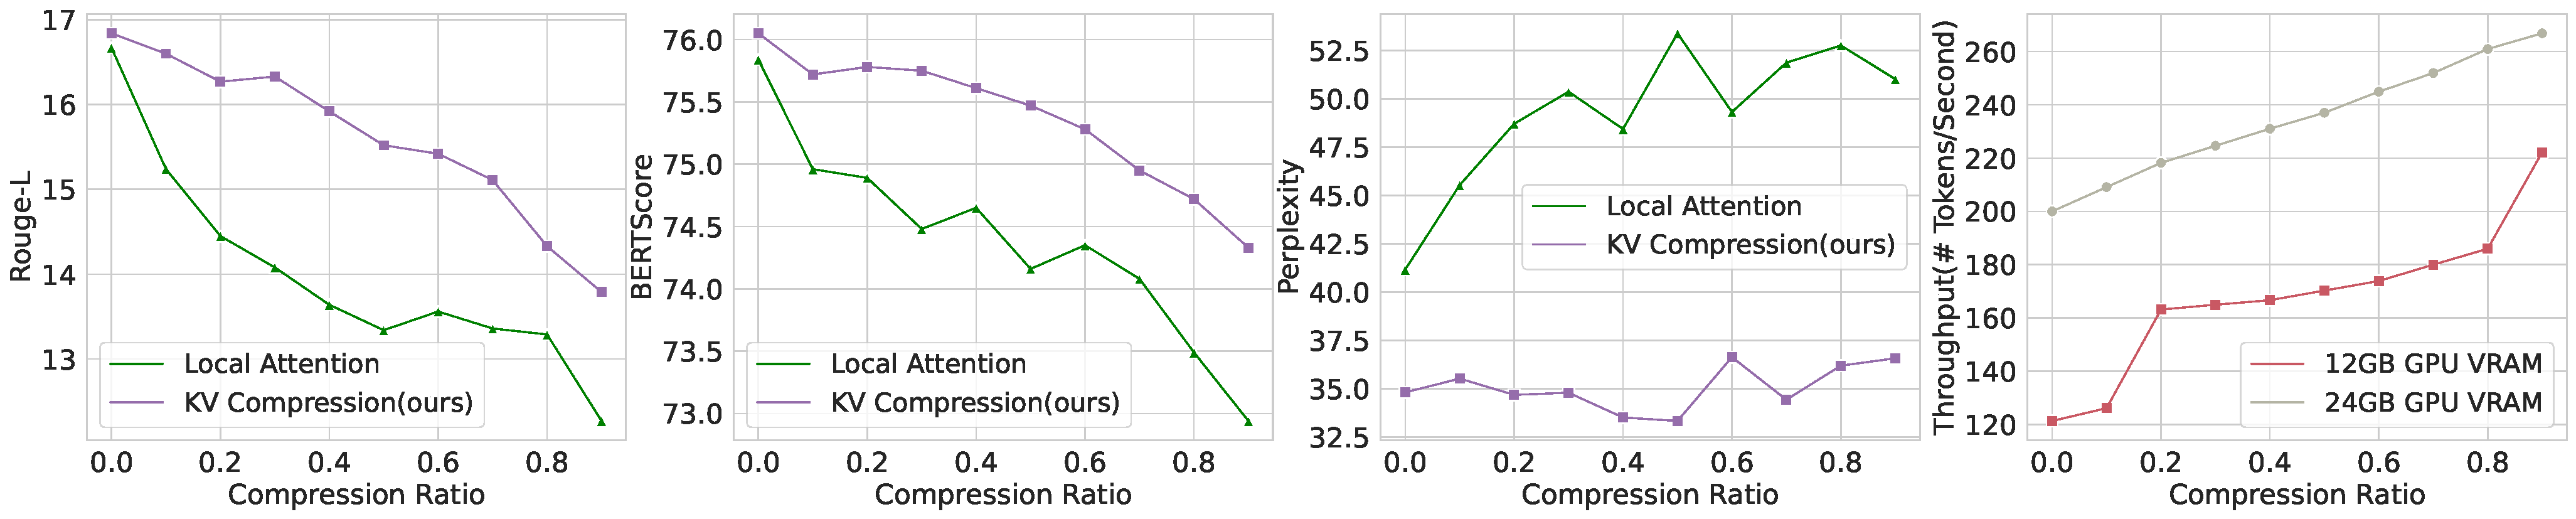
\includegraphics{./figures/redpajama3b_all.pdf}}
	\caption{RedPajama-3B on open-ended generation on 200 sampled C4 documents. Generation quality is measured by fluency~(perplexity), n-gram matching~(ROUGE-L), and semantic similarity~(BERTScore). We report system throughput as the number of tokens generated per second with different maximum GPU VRAM.
}
	\label{fig:open_ended}
\end{figure*}
\begin{table}[t]
	\small
	\centering
	\begin{tabular}{c|ccc}
	\toprule
	   \multirow{2}{*}{Method} & \multicolumn{3}{c}{Compression Ratio~($r$)}                                                                                                                                                                         \\
								                 & \multicolumn{1}{c}{0.7} & \multicolumn{1}{c}{0.8} & \multicolumn{1}{c}{0.9} \\
	\midrule
	 Local Attention       & 23.1                    & 25.2                    & 29.5                    \\
								  KV Compression      & \textbf{21.8}                    & \textbf{22.0}                    & \textbf{22.5}               \\    
	\bottomrule
	\end{tabular}
	\caption{Perplexity~(the lower the better) of RedPajama-3B  on WritingPrompts test set.
	}
	\label{table:WritingPrompts}
\end{table}
\subsection{Language Modeling}
\paragraph{Benchmark} We mainly conduct experiments on the Wikitext-2~\cite{wikitext2} dataset consisting of Wikipedia articles, which has been widely used for the evaluation of language modeling. We report token-level~(excluding \textit{<CL>} and \textit{<CR>} for KV Compression) average perplexity on the test set as the evaluation metric. We also report results on the WritingPrompts~\cite{wp} dataset to investigate the generality of our method.
\paragraph{Models} To demonstrate the generality of our approach, dubbed KV Compression, we adopt OPT-1.3B, OPT-2.7B~\cite{opt}, and RedPajama-3B~\cite{redpajama} as three LLMs with different sizes and position encoding methods.
\paragraph{Baselines} We compare our approach with two sparse attention baselines: (1) Scattered Attention which samples positions that permits attention from a Bernoulli distribution $\bm{B}(\text{1-}r)$; and (2) Local Attention~\cite{longformer} which restricts the attention of token $x_t$ to be within $(\lfloor t*r \rfloor,t)$. For KV Compression, we set $l$ as 25 throughout the experiments. Our proposed approach, alongside the sparse attention baselines we have selected, shares a common goal: enhancing the ratio of computation to memory access by curtailing the stored key-value cache. For detailed training setup please refer to Appendix \ref{appendix:detail}.
\paragraph{Results} The results on WikiText-2 are shown in \tabref{table:main}. As the compression ratio $r$ gets larger, all three methods result in an increase in perplexity either due to: (1) important tokens are out-of-scope for attention, or (2) the capacity of single \textit{<CR>} token is insufficient to encapsulate the full information of compressed token span. We observe that Local Attention substantially outperforms Scattered Attention, suggesting the importance of local context for language modeling. KV Compression achieves the best perplexity across various compression ratios. Notably, at high compression ratios, e.g., $r\geq 0.7$, KV Compression incurs significantly fewer degradation in perplexity compared to Local Attention, demonstrating its advantage in compressing scattered local information meanwhile keeping coherent global information. In \tabref{table:WritingPrompts}, we report the perplexity of RedPajama-3B on WritingPrompts dataset using Local Attention and the proposed KV Compression, with compression ratio from \{0.7, 0.8, 0.9\}. KV Compression achieves consistently lower perplexity compared to Local Attention, indicating its superiority as a domain-generalizable method for context compression.




\subsection{Zero-shot Open-ended Generation}
\label{sec:open}
\paragraph{Data} We randomly select 200 documents from C4~\cite{t5} validation set for evaluation. We use the leading 128 words as prefixes and treat the next 64 words as ground-truth references.
\paragraph{Models} We directly take the RedPajama-3B model trained on Wikitext-2 to perform zero-shot open-ended document generation. Given a prefix text $p$, nucleus sampling~\cite{topp} is used to generate a completion $c$ for it.
\paragraph{Baselines} Because Scattered Attention performs poorly according to \tabref{table:main}, we only compare KV Compression with Local Attention with compression ratio $r$ ranging from 0.0 to 0.9 applied to the prefix $p$ using input transformation defined in \secref{sec:kv} for KV Compression and restricted attention defined in \secref{sec:exp}. For Local Attention to achieve inference-time compression, it amounts to maintaining a FIFO queue to store the key-value cache: as the time step during generation increases, old key-value memory in the queue is popped out and newly generated key-value memory is pushed in.
\paragraph{Evaluation Metrics} We evaluate the quality of generated completions from three aspects: (1) fluency, (2) n-gram matching with ground-truth continuation, and (3) semantic similarity with ground-truth continuation. Fluency is evaluated by perplexity computed from Pythia-1B~\cite{pythia} model pre-trained using C4. N-gram matching and semantic similarity are measured by ROUGE-L and BERTScore~\cite{bertscore} respectively. To account for the randomness induced by nucleus sampling, for each prefix, we generate 8 completions and report the average results.
\paragraph{Results} \figref{fig:open_ended} shows that, as $r$ increases, the generated completions of Local Attention tend to diverge from the original topic, leading to decreased ROUGE-L/BERTScore and increased perplexity. Again, KV Compression excel at preserving relevant information and can still generate decent-quality continuations up to 0.5 compression ratio. Notably, KV Compression can generate fluent text even when the prefix is extremely compressed. The reason is that, during training, Local Attention receives rapidly faded information from the distant past, making the discourse structure for subsequent generations incoherent. On the contrary, KV Compression better preserve such information by consolidating it into sentinel tokens.

\subsection{Throughput Gain from Context Compression}
% The computation and memory intensity of the attention layer depends on both batch size $b$ and context length $L$. By reducing context length, it admits a larger batch size and improves the system throughput in return. To quantitatively measure the impact of context compression on throughput, we conduct experiments on open-ended generation by testing with different maximum available GPU VRAM. 
With KV Compression, the key-value cache corresponding to tokens enclosed by sentinel tokens can be freed from memory. In this way, it permits a larger batch size and improves the system throughput in return. To quantitatively measure the impact of context compression on throughput, we conduct experiments on open-ended generation by testing with different maximum available GPU VRAM. 
The full length of the dummy input prefix is set to 800 and we use RedPajama-3B with nucleus sampling to generate a continuation for it. The throughput of the text generation system is defined as the number of tokens generated per second. The results are shown in the bottom right of \figref{fig:open_ended}. We can see that, at extreme compression ratios~(e.g., $r\geq 0.8$), context compression offers more than 1.5x throughout improvement with 12GB GPU VRAM and a slightly smaller 1.3x improvement with 24GB GPU VRAM. 
At moderate compression ratio~(e.g., $r\approx 0.5$), KV compression is still able to deliver 1.2x-1.4x throughout improvement while only suffering from mild quality drop~(\secref{sec:open}). More visualized memory-compression ratio correlation is deferred to Appendix \ref{appendix:memory}.
